% Evaluation

\chapter{Evaluation} % Main chapter title

\label{Chapter6} % For referencing the chapter elsewhere, use \ref{Chapter4} 

\lhead{Chapter 6. \emph{Evaluation}} % This is for the header on each page - perhaps a shortened title

%----------------------------------------------------------------------------------------


\section{Quantitative}
\vspace{10pt}

\subsection{Evaluation of Mood Detection system}

\begin{figure}[t]
    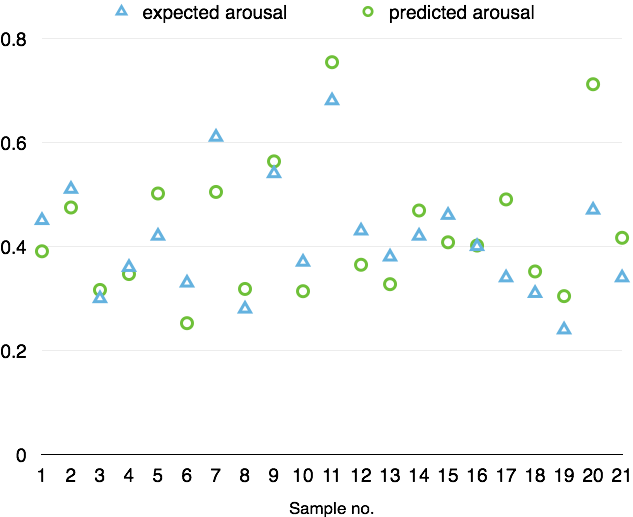
\includegraphics[width=0.7\textwidth]{Figures/finalarousal}
    \centering

  \caption{A plot of the expected and predicted .}
  \label{fig:anneval}
\end{figure}


We wanted to use neural networks to calculate valence and arousal ratings of songs using audio features we extract. 

We computed the mean error between participant ratings and network-predicted outputs across all segments of all test melodies. The network's performance total RMSE was 0.088954243616 on scale from 0 to 1. or 21.62\%.
The network predicted at an average accuracy of 78.38\% for all 20 segments. The plot of the expected and predicted values can be seen in Figure \ref{fig:anneval}.
These results are more promising than ones of Yang and Lin cite{mood}, where their $R^2$ scored 58.3\% for arousal and 28.1\% for valence.\textit{•}


\begin{figure}[t]
    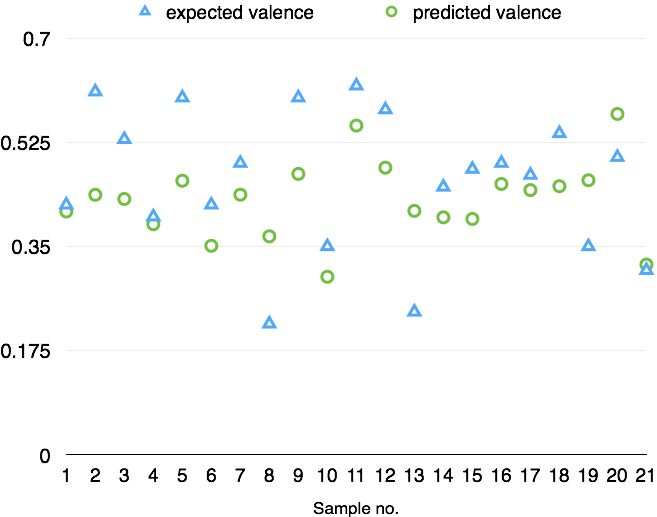
\includegraphics[width=0.7\textwidth]{Figures/finalvalence}
    \centering

  \caption{A plot of the expected and predicted .}
  \label{fig:anneval}
\end{figure}


Results from the static network indicate that a network can be trained to identify statistical consistencies across audio features abstracted from music and satisfactorily predict valence/arousal values that closely match mean participant ratings.


\begin{table}
\begin{center}
\begin{tabular}{| c | c | c | c | } \hline 
 expected arousal & expected valence & predicted arousal & predicted valence \\ \hline \hline

0.45  & 	0.42  &  0.390444 &  0.408524   \\ \hline
0.51	&  0.61  &  0.474538 & 0.436625   \\ \hline
0.3    &  0.53  &  0.316230 & 0.429643   \\ \hline
0.36	&  0.4    &  0.346713 & 0.387249   \\ \hline
0.42	&  0.6    &  0.501414 & 0.460295   \\ \hline
0.33	&  0.42  &  0.252398 & 0.350910  \\ \hline
0.61	&  0.49  &  0.504392 & 0.436785   \\ \hline
0.28	&  0.22  &  0.318096 & 0.366836   \\ \hline
0.54	&  0.6    &  0.563120 & 0.471717   \\ \hline
0.37	&  0.35  &  0.313782 & 0.298909   \\ \hline
0.68  &  0.62  &  0.753534 & 0.552922   \\ \hline
0.43	&  0.58  &  0.364568 & 0.482194   \\ \hline
0.38	&  0.24  &  0.327288 & 0.409628   \\ \hline
0.42  &  0.45  &  0.468762 & 0.398749   \\ \hline
0.46  &  0.48  &  0.407701 & 0.396029   \\ \hline
0.4    &  0.49  &  0.401469 & 0.454892   \\ \hline
0.34  &  0.47  &  0.490065 & 0.444592   \\ \hline
0.31  &  0.54  &  0.351714 & 0.451086   \\ \hline
0.24  &  0.35  &  0.304314 & 0.461078   \\ \hline
0.47	&  0.5    &  0.711224 & 0.572459   \\ \hline
0.34	&  0.31  &  0.416320 & 0.319491   \\ \hline


\end{tabular}
\caption{Table showing the root mean square error for training the network for given number of nodes in the hidden layer.}
\label{table:rsmetablefinal}
\end{center}
\end{table}


\subsection{Melody Extraction Testing}
To evaluate our implementation of the melody extraction algorithms we can use the technique used at Music Information Evaluation eXchange, described in section 2.4.3 of the report. In particular, we can compare the performance of our implementation when tested on the samples used during MIREX to the official statistics presented in papers \cite{salamon, comparison}.

Another way of evaluating the game is creating a set of songs and generating levels for them. After that a trained Guitar Hero player can play those levels. If the buttons were consistently on time with the notes then the melody extraction and game synchronisation techniques are considered to work.

\section{Qualitative}
Qualitative research is conducted to gain understanding of effects and benefit of the project. They focus on people's own experiences and provide insights and trends in thoughts on a given matter. They can be unstructured or semi-structured, conducted as group discussions, surveys or individual interviews.


\end{tabular}
\caption{Table presenting the results of the preliminary questionnaire.}
\label{table:preliminaryquestions}
\end{center}
\end{table}
What other features did you like in the game?
What other features were missing but you feel would be useful in the game?


\subsection{Questionnaires}
Questionnaires are one of the most common and popular tools to gather data from a large number of people. They generally consist of a limited number of questions that ask participants to rate the effectiveness of various aspects of the activity. The questions should focus on the key points we are trying to evaluate. 

Questionnaires tend to be short in order to reduce the amount of time respondents need to complete them, and therefore increase the response rate. 

We plan on writing questions that are quantitative and generally consist of close-ended questions (tick the box, or scales), as the open ended questions tent to make data analysis and reporting more difficult.


Before the design and implementation works, we conducted a study to determine what features could be desirable in the game. We conducted a survey among ====== FILL IN THE GAP ====== people aged  ======= FILL IN THE GAP ====== asking about their past experience with music rhythm games. 
The questions and the results are presented in the table below. Each of the questions was answered on a scale from 1 to 5, where 1 is a No,  3 is Neutral and 5 is a Yes.

\begin{table}
\begin{center}
\begin{tabular}{| p{8cm} | c | c | c | c | } \hline 
 Question & Average & Std. deviation & Min & Max \\ \hline \hline

Do you like playing games? & 2.5 & 2.5 & 2.5 & 2.5\\ \hline 
Do you like listening to music? & 2.5 & 2.5 & 2.5 & 2.5\\ \hline 
Do you often play games? & 2.5 & 2.5 & 2.5 & 2.5 \\ \hline 
Have you ever played Guitar Hero or other rhythm music game? & 2.5 & 2.5  & 2.5 & 2.5\\ \hline 
Did you feel like the choice of songs was limiting you? & 2.5 & 2.5 & 2.5 & 2.5 \\ \hline 
Were you able to load in your song of choice in there? & 2.5 & 2.5 & 2.5 & 2.5 \\ \hline 
Would you like to be able to load a song into it? & 2.5 & 2.5 & 2.5 & 2.5 \\ \hline 
Did you feel like the game graphics were reflecting the emotions in the song? & 2.5 & 2.5 & 2.5 & 2.5 \\ \hline 
Would you like the game to reflect the emotions in the song? & 2.5 & 2.5 & 2.5 & 2.5 \\ \hline 
Was the game reflecting the section of the song you were in? & 2.5 & 2.5 & 2.5 & 2.5 \\ \hline 
Do you feel it would be useful to know what section of the song is currently  played? & 2.5 & 2.5 & 2.5 & 2.5 \\ \hline 